\documentclass[10pt]{article}
\usepackage{graphicx} % Required for inserting images
\usepackage{geometry}
\usepackage[english,english]{babel}
\usepackage{blindtext}
\usepackage{lipsum}
\usepackage{parskip}
\usepackage{enumitem}
\usepackage{setspace}
\usepackage{caption}
\usepackage{multicol}
\usepackage{hyperref}
\usepackage{float}
\usepackage{changepage}
\usepackage{longtable}
\usepackage{multirow}
\usepackage{ragged2e}
\usepackage[style=apa,backend=biber]{biblatex}
\addbibresource{referencias.bib}

\usepackage{parskip}

\usepackage{booktabs}


\usepackage{tikz}

\usetikzlibrary{shapes, arrows}
\usetikzlibrary{shapes.geometric}
\usetikzlibrary{positioning}
\usetikzlibrary{positioning, arrows.meta}
\usetikzlibrary{shapes, arrows.meta}

\tikzstyle{block} = [rectangle, draw, fill=blue!20, text width=6em, text centered, rounded corners, minimum height=3em]
\tikzstyle{line} = [draw, -latex']
\tikzstyle{cloud} = [draw, ellipse, fill=red!20, node distance=3cm, minimum height=2em]

\usepackage{schemata}
\usetikzlibrary{mindmap}

\usetikzlibrary{fit,positioning}

\geometry{
    top=2.5cm,
    left=2.8cm,
    right=2.8cm,
    bottom=2.44cm
}

\tikzset{
every picture/.append style={
  execute at begin picture={\deactivatequoting},
  execute at end picture={\activatequoting}
  }
}

\usepackage{titlesec}

\titleformat{\section}{\fontsize{10}{12}\selectfont\bfseries\centering}{\thesection. }{1em}{}
\titlespacing*{\section}{0pt}{\baselineskip}{\baselineskip}

\titleformat{\subsection}{\fontsize{10}{12}\selectfont \itshape}{\thesubsection. }{1em}{}
\titlespacing*{\subsection}{0pt}{\baselineskip}{\baselineskip}

\titleformat{\subsubsection}{\fontsize{10}{12}\selectfont \itshape}{\thesubsubsection. }{1em}{}
\titlespacing*{\subsubsection}{0pt}{\baselineskip}{\baselineskip}

\usepackage[pages=all]{background}

\backgroundsetup{
 scale=1, %escala de la imagen, es recomendable que sea del mismo tamaño que el pdf
 color=black, %fondo a usar para transparencia
 opacity=0.2, %nivel de transparencia
 angle=0, %en caso de querer una rotación
 contents={%
  
\includegraphics[width=\paperwidth,height=\paperheight]{template1.pdf} 
 }%
}

\usepackage{fontspec}
\setmainfont{Times New Roman}

\title{\vspace{0cm} \fontsize{10}{12}\selectfont \textbf{Credit Card Approval Prediction Research Using Predictive Modelling} 

\vspace{4mm} }
\author{\fontsize{10}{12}\selectfont \textbf{\fontsize{10}{12}\selectfont Rajesh Goldy under supervising of PhD. Shagufta Henna} \\ \\
\small{\textbf{\fontsize{10}{12}\selectfont Atlantic Technological University}}\\
\small{\fontsize{10}{12}\selectfont Port Rd, Gortlee, Letterkenny, Co. Donegal}\\
 \\ \small{\fontsize{10}{12}\selectfont Tel.: (074) 918 6000}\\
\small{\fontsize{10}{12}\selectfont Web: \ www.lyit.ie}}
\date{\vspace{-6mm}}

\begin{document}

\fontsize{10}{12}\selectfont

\selectlanguage{english}

\def\tablename{Tabla}%

\setlength{\parskip}{0mm}

\maketitle

\setlength{\parskip}{3mm}

\selectlanguage{english}

\renewcommand\abstractname{}

\begin{abstract}
    \fontsize{10}{12}\selectfont
    \textbf{Abstract:} This research project discusses the factors affecting credit scores, a crucial tool for risk management in the financial domain. The decision to issue a credit card depends upon various factors, including the client's age, salary, and credit score. Economic conditions also play a significant role, as financial firms may face higher rates of default during economic downturns. After performing statistical analysis, this project aims to develop an understanding of a client’s behavior by analyzing attributes and the weight carried by it in predicting whether a credit could be a bad or good credit. 

    \vspace{3mm}
    
    \textbf{Keywords:} Credit Card, Predictive Modelling, Risk, Handling missing values, Ensemble Method
    \vspace{-7mm}
\end{abstract}

\selectlanguage{english}

\renewcommand\abstractname{}

\begin{abstract}
    \fontsize{10}{12}\selectfont
    \textbf{Summary:} 
    This project revolved around in-depth exploration of a credit-related dataset from Kaggle, comprising credit and application records. It leveraged vintage analysis, data visualization and correlation evaluation. The data preprocessing techniques like handling missing data with machine learning model, PCA, t-SNE, Standard Scaler and Smote are incorporated to enhance the predictive capability of the model’s performance. This work is implemented in Python and performance is evaluated using primary and guard-rail metrics like F1 and (Balanced Accuracy and Precision Score) respectively. SVM most performed among all other model and scored 77\% on F1, a balanced accuracy of 62\%, and precision of 72\% on test data.
    
    \vspace{3mm}
    
\end{abstract}

\vspace{3mm}

\setlength{\columnsep}{1cm}

\renewcommand{\tablename}{Tabla}

\begin{multicols}{2}\
\fontsize{10}{12}\selectfont

\section{Introduction and Motivation}

In 2008 global economic crisis occurred, also known as The Great Recession, which impacted a lot of lives. At its core, the Great Recession was ignited by banks that issued a significant number of credit cards at an alarming rate, leading to an increase in default rates. Financial institutes then agree to regulate the environment to provide credit cards to users based on their historical patterns (good credit or bad credit). Although their defined set of rules needs to be altered based on the current market situation. For instance, an economic fluctuation (like COVID-19) impacted the economic behavior (earning and expenditure rate) of personnel thus creating an impact on the repayment of loans.
The goal of this project is to investigate: 
1.	The impact of attributes on client status
2.	Discover the attributes responsible for the client’s default
3.	Training a model to classify the data points into a good or bad credit

The study utilizes the data from Kaggle named “Credit Card Approval Prediction”, initially a machine learning model is trained to predict the missing values in a column “Occupation type” and at last by using multiple supervised machine learning algorithms a final model is picked using hyperparameter tuning to predict the behavior of a client. The model showcases the feature selection using statistical analysis as well as machine learning methods. 
}

\section{Dataset Overview}

The data used in credit card research and predicting a model is taken from Kaggle an open-source platform for datasets. The directory consists of 2 files named credit-record.csv and application-record.csv. The metadata of credit\_record.csv incorporates features: ID, Gender, Own's car, Own's realty, count of children, income amount, category of income, marital status, housing type, age, day's employed, mobile, work phone, email, occupation type, count of family memebers. 

The metadata of application\_record.csv is given below:

\begin{itemize}[itemsep=0pt]
    \item ID: ID associated with a client
    \item MONTHS\_BALANCE: The month of the extracted data is the starting point, backward, 0, is the current month, 01 is the previous month, and so on
    \item STATUS: 0: 1-29 days past due, 1: 30-59 days past due, 2: 60-89 days overdue, 3: 90-119 days overdue, 4: 120-149 days overdue, 5: Overdue or bad debts, write-offs for more than 150 days C: paid off that month X: No loan for the month
    \end{itemize}

There is a total of 438557 records in the credit\_score.csv, where application\_record has 1048575 records. Unique values in application\_record is 45985 i.e. data of a client in application\_record is repeating and captured the behavior for a certain time.


\section{Vintage Analysis}

In credit risk, it is a popular method for managing credit risk. The term 'Vintage' refers to the month or quarter in which account was opened (loan was granted). In simple words, the vintage analysis measures the performance of a portfolio in different periods of time after the loan (or credit card) was granted. Performance can be measured in the form of cumulative charge-off rate, proportion of customers 30/60/90 days past due (DPD). To generate the label, the credit’s status is summed together, if the overall credit’s status is greater than 0 it is marked as 1(bad credit) otherwise labeled as good credit (label 0). 

\section{Data Exploration}
The newly generated labels (in application\_records.csv) are joined to the credit\_score.csv dataset. Fig 1 illustrates the visual representation of the good vs bad credit in terms of the ratio. 
\vspace{-3mm} 
\begin{figure}[H]
    \centering
    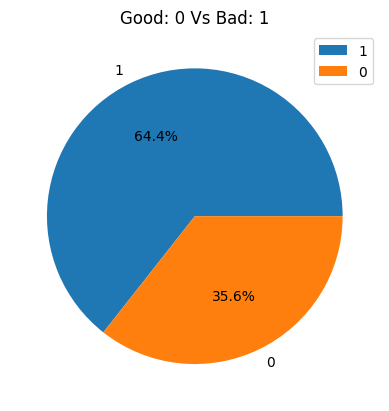
\includegraphics[width=1\linewidth]{fig1.png}
    \caption{\justifying \textit{Distribution of Good vs Bad credit}}
    \label{fig:PID Fuzzy}
\end{figure}
\vspace{-5mm} 
Only 35.6\% of the users hold good credit status and 64.4\% falls under bad credit category. \\ \newline \newline Figure 2 depicts the information about the null values in the dataset, where “occupation type”, “status” and “labels”(new labels) are null. 

\begin{figure}[H]
    \centering
    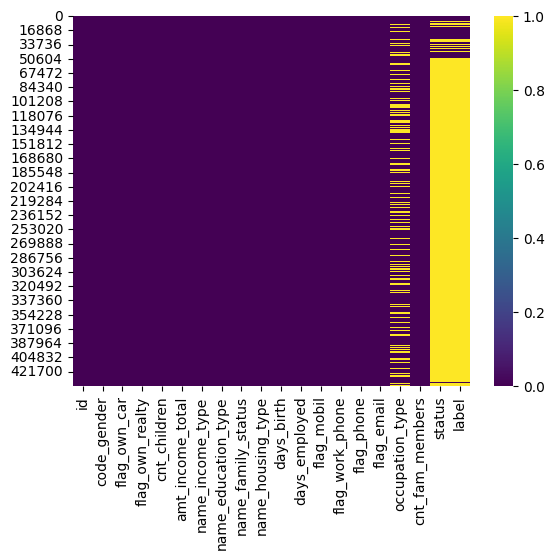
\includegraphics[width=1\linewidth]{fig2.png}
    \caption{\justifying \textit{Heatmap: Null values}}
    \label{fig:PID Fuzzy}
\end{figure}

\begin{figure}[H]
    \centering
    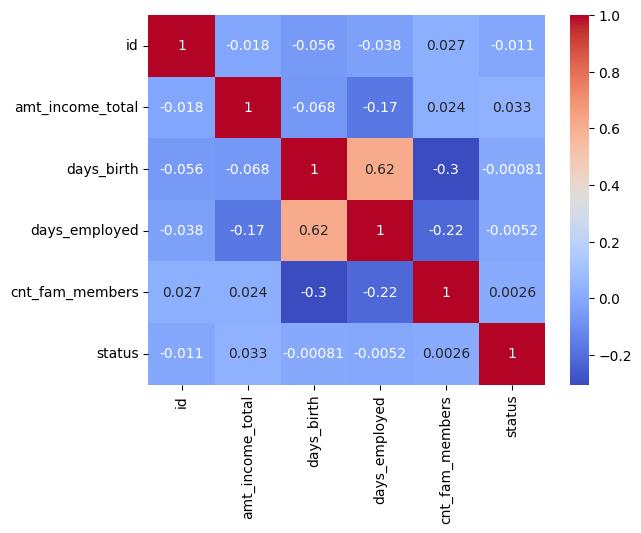
\includegraphics[width=1\linewidth]{figure3.png}
    \caption{\justifying \textit{Pearson Correlation}}
    \label{fig:PID Fuzzy}
\end{figure}

Figure 3 shows the plot of the correlation of all continuous variables with respect to each other. To calculate the correlation between continuous variable “Pearson” method is used, the value of Pearson correlation ranges from -1 to 1, where +1 indicates a strong positive correlation and -1 interprets that 2 continuous variable is strongly correlated to each other but in a negative direction. 0 means no correlation. And in credit risk, the interesting thing to note is that “annual income is negatively correlated to the days employed (-0.17)”. Days employed and days of birth (age) are positively correlated with each other at 0.62. For the categorical variables, hypothesis testing is performed, and Mann Whitney test is used to check the relation with the target variable (good or bad) at a 95\% confidence interval. In analysis, it has been found that Occupation type and education have an impact on the target variable at a 95\% confidence interval, whereas the rest of the variables like having a work phone, email, family status, and gender have no significant impact on predicting whether the client will cause delays in repaying the loan on time or not. 

\section{Treating missing values}
Given that 30\% of data in the occupation type attribute is missing; it proposed a significant challenge.  If filled with the most common value (mode) might cause the model to be trained biased as occupation type has significant on predicting the target variable (from statistical analysis). Therefore, a machine learning model is trained to predict the occupation type. Initially, Random Forest model is trained with default parameters and training score reached to 0.52 and test score was 0.48, but with hyperparameter tuning {max\_depth:None, min\_samples\_lead:1, min\_samples\_split: 2, n\_estimators: 200} on Random Forest; train score reached to 0.98 where test score is 0.92.
\begin{figure}[H]
    \centering
    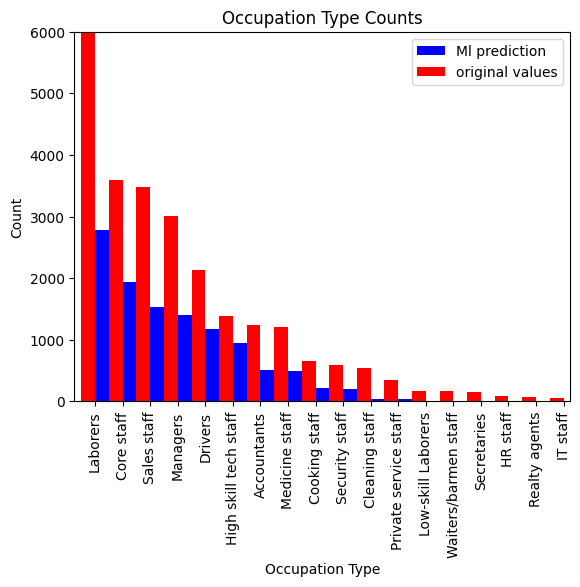
\includegraphics[width=1\linewidth]{figure4.png}
    \caption{\justifying \textit{Pearson Correlation}}
    \label{fig:PID Fuzzy}
\end{figure}

Figure 4 illustrates the original distribution of occupation types (shown in red) alongside the proportion of all other occupation types predicted by the random forest model (shown in blue). An intriguing observation from this visualization is that the distribution of predicted values across various categories closely resembles the distribution of the original values.

Figure 5 depicts the top 5 features that are crucial in predicting the occupation type.  
\begin{figure}[H]
    \centering
    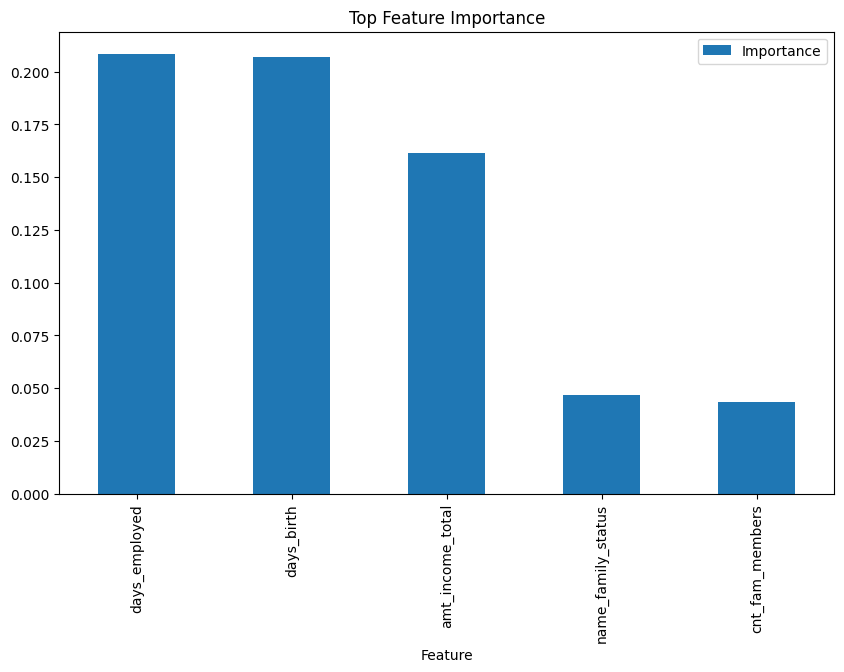
\includegraphics[width=1\linewidth]{figure5.png}
    \caption{\justifying \textit{Pearson Correlation}}
    \label{fig:PID Fuzzy}
\end{figure}


\section{Overview of practice used}
This paper leverages the strategies of pre-processing techniques like Principal Component Analysis (PCA), t-Distributed Stochastic Neighbor Embedding (t-SNE), Standard Scaler, and Synthetic Minority Over-sampling Technique (SMOTE). These techniques plays crucial role in enhancing the model’s performance, visualizing the data and solving problems like imbalance dataset. 

\subsection{PCA: Principal Component Analysis}
PCA is a dimensionality reduction technique designed to transform high-dimensional data into a lower-dimensional space while retaining its essential features. It works by calculating the variance against all dimensions which are essential to explain the variance in the dataset. Having higher dimensions in training dataset might result in curse of dimensionality and PCA eliminates the noise in dataset thus increasing the model’s performance by eliminating the noisy data. This research paper selected the number of components required to build the model by visualizing the graph given Fig 6

\begin{figure}[H]
    \centering
    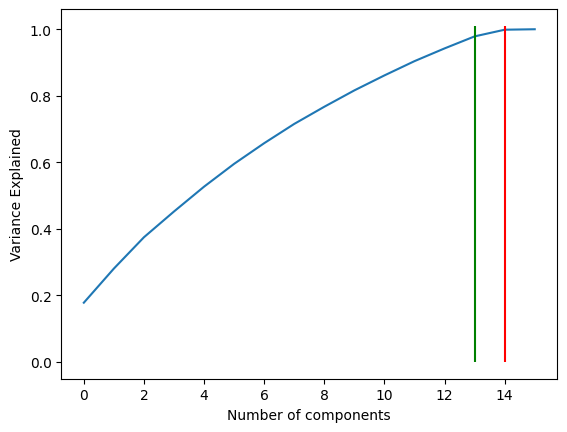
\includegraphics[width=1\linewidth]{figure6.png}
    \caption{\justifying \textit{PCA}}
    \label{fig:PID Fuzzy}
\end{figure}
From the above graph, 13 or 14 components are required to explain the whole variance present in the dataset. 

\subsection{t-Distributed Stochastic Neighbor Embedding (t-SNE)}
t is a nonlinear dimensionality reduction method that excels in visualizing high-dimensional data in lower-dimensional spaces. Emphasizing the preservation of pairwise similarities, t-SNE unveils intricate patterns and structures within data. The paper elucidates the algorithmic principles of t-SNE, its applications in exploratory data analysis, and considerations for optimal implementation. Fig 7 aids in visualizing the higher dimensional data into 3 dimensions. From the graph, it can be concluded that predicting whether a credit will be good or bad can be challenging for the machine learning models with 100\% accuracy.

\begin{figure}[H]
    \centering
    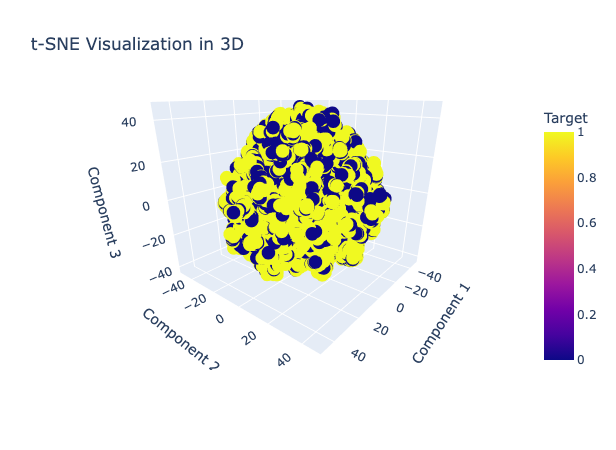
\includegraphics[width=1\linewidth]{figure8.png}
    \caption{\justifying \textit{PCA}}
    \label{fig:PID Fuzzy}
\end{figure}


\subsection{Standard Scaler}
It is a pre-processing technique designed to transform and standardize the features of a dataset. Standardization is crucial in scenarios where features have different scales, as it ensures that all features contribute equally to the analysis.
The standardization process involves transforming the data in such a way that it has a mean of 0 and a standard deviation of 1. This is achieved by subtracting the mean of each feature and then dividing by its standard deviation. The formula for standardization of a feature is given below:
\newline
\newline
$X_{\text{standardized}} = \frac{X - \text{mean}(X)}{\text{std}(X)} $

Here, mean(x) represents the mean of the feature, and std(x) represents its standard deviation. Standardization is particularly beneficial for algorithms that rely on distance-based calculations, such as k-nearest neighbours or support vector machines.


\subsection{SMOTE}
To determine the optimal number of clusters for implementing the SMOTE algorithm, an unsupervised machine learning approach using "K-Means" was used. Figure 8 plots the elbow method and Silhouette Score, which are common utilized methods to identify the number of clusters in a dataset. However, in this case, there is no distinct elbow point visible, making it challenging to determine the number of clusters identified by the K-Means algorithm in the dataset.

\begin{figure}[H]
    \centering
    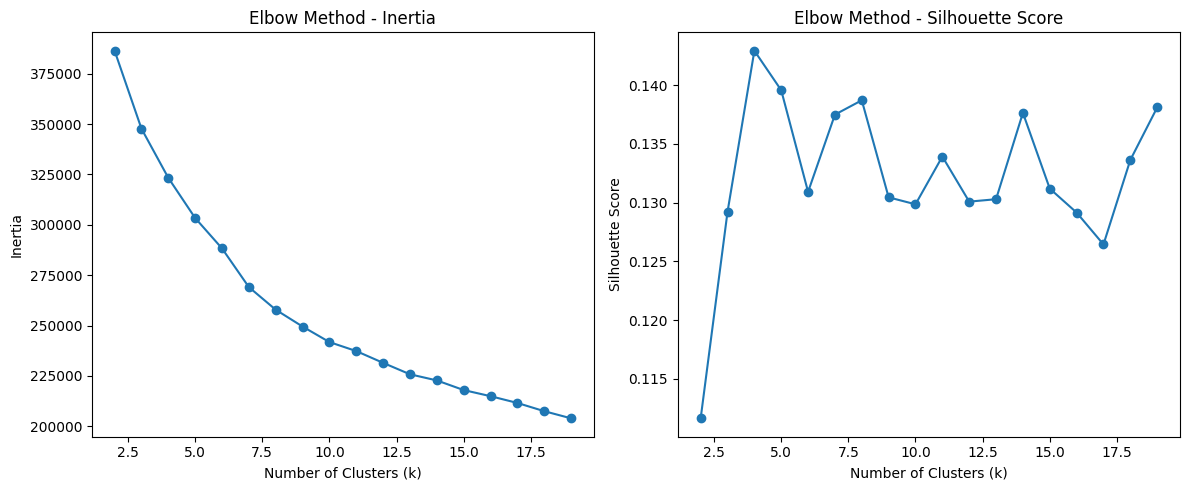
\includegraphics[width=1\linewidth]{figure9.png}
    \caption{\justifying \textit{PCA}}
    \label{fig:PID Fuzzy}
\end{figure}


\section{Training Model}
\subsection{Criteria for performance accuracy: }
The primary evaluation metric for the model is the F1 score, a harmonic mean of precision and recall, while the balanced accuracy serves as the guardrail metric. True Positive (TP) and True Negative (TN) values indicate correct predictions for 'good credit' and 'bad credit,' respectively. False Positive (FP) and False Negative (FN) represent incorrect predictions. Balanced Accuracy, derived from the average of True Positive Rate (TPR) and True Negative Rate (TNR), offers a relatively fair evaluation of the model's performance.

\begin{left}
\begin{tabular}{c|c|c}
\multicolumn{1}{c}{} & \multicolumn{2}{c}{\textbf{Predicted}} \\
\cline{2-3}
\multicolumn{1}{c|}{} & \textbf{Positive} & \textbf{Negative} \\
\hline
\textbf{Actual Positive} & TP &  FN \\
\hline
\textbf{Actual Negative} & FP & TN \\
\end{tabular}
\end{left}

\section*{True Positive Rate (Sensitivity, Recall)}

\[
TPR = \frac{TP}{TP + FN}
\]

\section*{False Positive Rate}

\[
FPR = \frac{FP}{FP + TN}
\]

\section*{F1 Score}

\[
F1 = \frac{2 \cdot \text{Precision} \cdot \text{Recall}}{\text{Precision} + \text{Recall}}
\]


\subsection{Random Forest Classifier}
It is an ensemble learning method that constructs multiple decision trees during training and output the mode (in case of classification) or mean prediction (in regression) of the individual tree. By aggregating the prediction of multiple trees, Random Forest increase the predictive accuracy and generalization of unseen data; however, this algorithm is having a higher tendency to overfit the data if not tuned properly. In this research, RFC (Random Forest Classifier) is trained in several ways, initially it is trained on the whole dataset and 	 the columns that RFC indicates most important for predicting the results as shown in Figure 9. After retraining the model on import features like "days\_birth", "days\_employed",
                              "amt\_income\_total", "occupation\_type", "name\_family\_status", "name\_income\_type" the training score increased from 0.83\% to 0.84\% and where test score showed no improvement and remained stable at 0.73\% on train and test dataset. 

\begin{figure}[H]
    \centering
    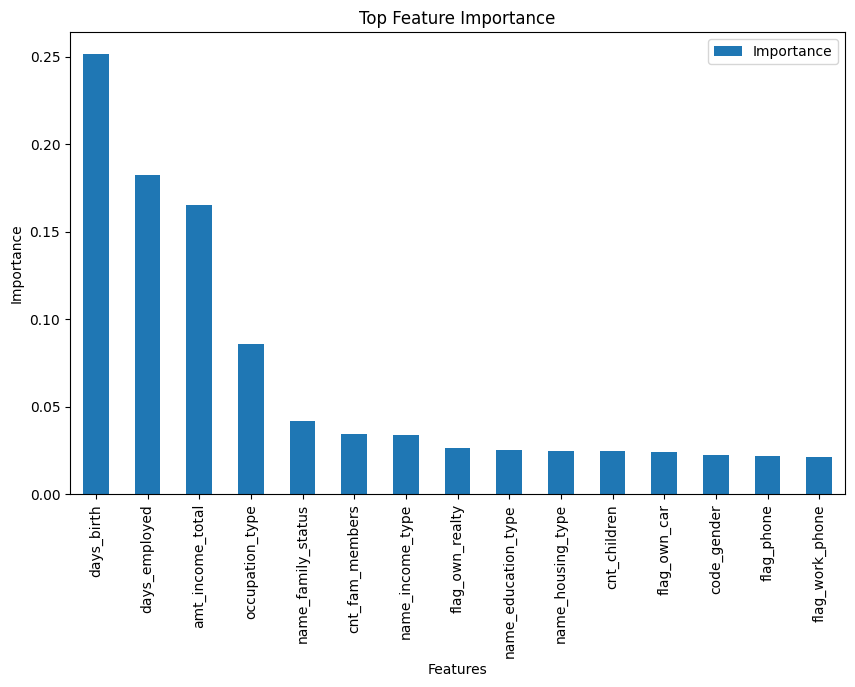
\includegraphics[width=1\linewidth]{figure10.png}
    \caption{\justifying \textit{Feature Importance}}
    \label{fig:PID Fuzzy}
\end{figure}

\subsection{Support Vector Machine}
It is a powerful supervised machine learning algorithm used for classification and regression tasks. The primary objective of SVM is to find a hyperplane in an N-dimensional space (where N is the number of features) that distinctly classifies data into different categories. SVM is particularly effective in high-dimensional spaces, making it suitable for complex data. As seen in t-sne visualization in figure 7, it is clear that dataset is not linearly separable making SVM as a perfect choice for this classification project. Although it is efficient for linear classification as well; however, the time taken by this algorithm is high. Model is trained on whole dataset with default set of parameters and sucessfully scored 0.85\% f1 score on training dataset and 0.77\% on test data. 

\subsection{XGBOOST}
It stands for Extreme Gradient Boosting works for both classification and regression tasks. It combines predictive accuracy of weak learner, typically decision trees to create a robust model. It operates by adding decision trees to correct errors made by previous model resulting low error at last model. This algorithm is not a part of scikit-learn but a different open-source package. The algorithm support learning rate a hyper-parameter (learning rate) to converge to the minimum loss, where other algorithm has default settings. 
In this research, the model f1 score on training data (without PCA and standard scaler) is 79\% and on test dataset is 0.77\% which shows the model is not doing overfitting compared to other 3 models trained. 



\section{Results}
After experimenting with different models and deploying several techniques, it was observed that Support Vector Machine (SVM) yielded the best results when trained on important features selected by Random Forest Classifier. SVM achieves an amazing F1 score of 77\%, a balanced accuracy of 0.62\% and precision of 0.72\% on test data. Based on primary metric F1 score model can predict whether a credit is good or bad at 77\% confidence level. 
No significant difference is measured when SVM compared with Random Forest and XGBoost classifier; however, the F1 score of SVM results in a 5.48\% improvement in achieving a balanced trade-off between precision and recall. Table 2 presents the model’s accuracy after tuning with hyperparameters.

\begin{table}[H]
    \centering
    \caption{\textit{Model Performance on whole dataset}}
    \begin{tabular}{cccccc}
        \hline
         & \textbf{F1} & \textbf{BA} & \textbf{Precision}\\
        \hline
        \textbf{Train Score}\\
        \textbf{RFC} & 0.83 & 0.80  & 0.88\\
        \textbf{SVM} & 0.85 & 0.76  & 0.80\\
        \textbf{XGB} &  0.82 & 0.77 & 0.69 \\
        \textbf{Test Score}\\
        \textbf{RFC} & 0.73 & 0.65  & 0.76 \\
        \textbf{SVM} & 0.77 & 0.62  & 0.72 \\
        \textbf{XGB} & 0.66 & 0.59  & 0.67\\
        \hlines
    \end{tabular}
    \label{tab:Base de Reglas}
\end{table}

\section{Conclusion}
This project offered an amazing opportunity for obtaining hands-on experience in predictive modelling and experimenting with different techniques to train a model. Choosing python and it’s library like sklearn, plotly, matplotlib, xgboost showed the excellent opportunities in making a smart decision. Using pandas to handle the data and filling missing values using machine learning model provided a excellent method in cleaning the dataset rather than naively filling huge percentage of missing data with mode or mean. 

This project utilized a dataset sourced from Kaggle, consisting of credit record and application record files. The exploration and analysis involved vintage analysis to generate labels, data exploration visualizations, and correlation assessments. The data preprocessing pipeline uses techniques such as Principal Component Analysis (PCA), t-Distributed Stochastic Neighbor Embedding (t-SNE), Standard Scaler, and Synthetic Minority Over-sampling Technique (SMOTE). The predictive modeling phase employed Random Forest Classifier, Support Vector Machine (SVM), and XGBoost algorithms, with SVM emerging as the top performer. SVM's superior F1 score of 77\%, balanced accuracy of 62\%, and precision of 72\% on the test data, showcasing its effectiveness in predicting credit status. This research contributes valuable insights into credit risk management and the application of machine learning techniques for enhanced predictive modeling.

\section{References}


\item XGBoost: \href{xgboost}{https://medium.com/analytics-vidhya/introduction-to-xgboost-algorithm-d2e7fad76b04}
\item Random Forest: \href{Random Forest}{https://www.analyticsvidhya.com/blog/2021/10/an-introduction-to-random-forest-algorithm-for-beginners/}
\item Scikit-learn: \href{Scikit-learn}{https://scikit-learn.org/stable/supervised\_learning.html}

\end{document}
